\documentclass [paper]{ieice}
\usepackage {cite}
\usepackage{graphicx}
	\graphicspath{{images/}}
\usepackage {latexsym}
\usepackage [varg]{txfonts}
\usepackage[none]{hyphenat}%%%%

\setcounter{page}{1}

%local definitions
\def\ClassFile{\texttt{ieice.cls}}
\newcommand{\PS}{{\scshape Post\-Script}}
\newcommand{\AmSLaTeX}{%
 $\mathcal A$\lower.4ex\hbox{$\!\mathcal M\!$}$\mathcal S$-\LaTeX}
\def\BibTeX{{\rmfamily B\kern-.05em
 \textsc{i\kern-.025em b}\kern-.08em
  T\kern-.1667em\lower.7ex\hbox{E}\kern-.125emX}}
\hyphenation{man-u-script}
\makeatletter
\def\tmpcite#1{\@ifundefined{b@#1}{\textbf{?}}{\csname b@#1\endcsname}}%
\makeatother
%end local definitions

\field{A}
\vol{01}
\no{01}

\title {Industry Application of Software Development Task Measurement System : TaskPit}
%\titlenote{This paper was presented at ...}

\authorlist{
 	\authorentry{Pawin Suthipornopas}{}{labelA}
 	\authorentry{Pattara Leelaprute}{}{labelA}
	\authorentry{Akito Monden}{}{}
	\authorentry{Hidetake Uwano}{}{}
	\authorentry{Yasutaka Kamei}{}{}
	\authorentry{Kenji Araki}{}{}
	\authorentry{Kingo Yamada}{}{}
	\authorentry{Ken-ichi Matsumoto}{}{labelB}
}
\affiliate[labelA]{Department of Computer Engineering, Kasetsart University}
\affiliate[labelB]{Nara Institute of Science and Technology}

\author{Pawin Suthipornopas,
		Pattara Leelaprute, \\
		Akito Monden, 
		Hidetake Uwano, 
		Yasutaka Kamei, \\
		Kenji Araki, 
		Kingo Yamada, 
		Ken-ichi Matsumoto}
		


\date {2015-07-07}

\begin {document}

\maketitle
\begin {summary}
	Introduction of software development process measurement into industry level of software development using TaskPit with little requirements and less cost in implementing with the industry level. Contains two study cases, one is a group of developers measured in approximately a week of business days with normal method of measurement resulted in some improvements capability. Another study case is a single developer measured by TaskPit resulted in an active improvement in completing unplanned work in limited time. 
\end {summary}

\section {Abstract}
	To find any problems in a software development process, we have been developing an automated measurement tool called TaskPit, which monitors software development tasks such as programming, testing and documentation based on the execution history of software applications. This paper introduces the system requirements, design and implementation of TaskPit; then, presents two industry case studies applying TaskPit to actual software development. In the first case study, we applied TaskPit to 12 software developers in a certain software development division. As a result, several concerns (to be improved) have been revealed such as (a) a project leader spend too much time on development tasks while he was supposed to be a manager rather than a developer, (b) several developers rarely used e-mails while a company instructed developers to use e-mails as much as possible to leave communication records during development, and (c) several developers wrote too long e-mails to their customers. In the second case study, we have recorded the planned, actual, and declared time of development tasks. As a result, we found that (d) there were unplanned tasks in more than half of days, and (e) the declared time became closer day by day to the actual time measured by TaskPit. These suggest that TaskPit is useful not only for a project manager who is responsible to the process improvement but also for a developer who wants to improve by him/herself.
\section {Introduction}
	
	To promote an idea of "Process Improvement via Measurement" in software industry, we had developed a software development task measurement system called TaskPit\cite{taskpit} in 2008, and have been updating it till today. TaskPit automatically records the time and the amount of work of daily tasks of an individual developer or a development team to find any problems in software development. It can record the time spent for each task such as "Programming" using Eclipse or Visual Studio, "Documentation" using Word or other text editors, "E-mail" using Gmail on a browser and so on, where a task is associated with a set of applications and window titles. TaskPit records an amount of work for each task in terms of the number of keystrokes and the mouse clicks. It can also records an amount of deliverables of each task as the increased size of files in a directory associated to the task. \par
	To date, the TaskPit community has been gradually grown up, user manuals and related tools have been developed by volunteers, and as of July 2015, total downloads of TaskPit version 1.0.0 to 1.0.3 has reached 1500\cite{taskpit}. Now we are demanding for industry case studies to share the experience and findings about how TaskPit could be used for process improvement. \par
	This paper introduces the system requirements, design and implementation of TaskPit; then presents industry case studies applying TaskPit to two software organizations. The first organization consists of 12 members, measured in 9 days (6 business days) where 7 are developers, 3 leaders, and 2 customer services. Analysis of data and measurements of the work surveyed in departments are collected and summarize by one veteran employee from other department to look after the flow of their work. In the second organization there is only one developer measured in 17 days (13 business days) measured by TaskPit. In addition to the automatic measurement TaskPit did, there is also a value plan and engage time for each development tasks for this developer each day. This is to clarify the difference between the measured value that was collected and analyze manually, and automatic measurement. \par
	Please note that this paper is an extension of our Japanese workshop paper (short paper) [FOSE2013] with an additional (second) case study. In this paper we also added explanations of the system requirements, design and implementation of TaskPit to clarify the design concept of TaskPit and to illustrate how TaskPit can be used in software organizations. \par
	In the following Chapter 2, we will describe the related work and research in background, Chapter 3 will be about TaskPit and its system requirements, design, and implementation. In Chapter 4 and 5 will be measurement results and analysis in two organizations. Lastly in Chapter 6 is a summary.
	
\section {Background and Related Work}
	
	As Tom DeMarco said 「You can't control what you can't measure」we believe it is essential to control the process of developing software\cite{demarco1986controlling}. For this purpose, various product processes metrics and measurement have been applied to the developing site\cite{grady1992practical}. In many of the environment of development site; the software scale, work hours, and bugs are measured and used for project management, and quality assurance of the development\cite{nec2010software}\cite{putnam2013five}. \par
	On the other hand, problems found in the development field are mostly from human factors\cite{sec2010itproject} rather than the product process and measurements. This is considered to be natural as described in Personal Software Process (PSP) and Team Software Process (TSP), where developers and the development team follow up the work of day-to-day tasks and record everything manually, these methods are well-known as a method for process improvement\cite{humphrey1995discipline}\cite{humphrey2001}. However, as developers have to do this manually, this method popularity grows thin and does not spread widely as it should. \par
	At first, PSP has been proposed as a measurement procedure in accordance with a specific measurement form which required accurate calculation and required great cost to the data measurement. There are also tools and systems that act as a supporting role in data measurement to help calculating data more easily such as Process Dashboard\cite{processdashboard}, Task Coach\cite{taskcoach} and Slim Timer\cite{slimtimer}, but using these tools will required to switch the measurement work (Context Switching) because they are all in different environment, and this has become a barrier in introducing the measurement procedure to the development site\cite{sillitti2003collecting}. \par
	Without causing the Context Switch, automatic measurement tools on software development have been proposed, for example EPM\cite{ohira2004empirical}, Ginger\cite{}, Ginger2\cite{torii1999ginger2}, HackyStat\cite{}, and PROM\cite{}. Detailed data collected by these tools can be used with less cost. \par
	In this paper, the main objective is to support the introduction of process improvement in the development team. It is easy to introduce TaskPit as a system that does not require pre-planning, and capable of carrying out process improvement through measurement. TaskPit will record the number of hours and amount of work separately task by task, and can automatically measure the changes in the result number compared to actual number. Data in the system is to measure the amount of work, and achievement in each task are directly represents and are easily analyzed. It is suitable for the stage of process improvement during development.
	
\section{TaskPit}

\subsection{System Requirements}
	Based on the previous chapter of this paper and the requirements of task measuring system, our system requirements are described in detail in the following subsection: \par
	
\subsubsection{[Requirement 1: Binding between Tasks and Applications]}
	In TaskPit system, each development task are to be work on different applications and windows. Therefore, we need to bind the task name with application name corresponding to it (the executable file name or process name). However, in the actual work, it is not always necessary to use only one application to perform one task. One application might work on many tasks, and one task might be completed by many applications. Moreover, even in different tasks, it may use the same application. In such a case, to distinguish tasks by differences in the character string in the name of the window during application execution, we approach it with BNF as follows: \par

\begin{itemize}
	\item[] $\langle$Task$\rangle$ ::= $\langle$Application$\rangle$ \{$\|$$\langle$ Application $\rangle$\}
	\item[] $\langle$Application$\rangle$ ::= $\langle$Executable File Name$\rangle$ [$\langle$Window Name$\rangle$]
\end{itemize}

	Tasks are defined as a set of one or more running applications, and applications are defined as a set of executable name and window name. Below are examples of how tasks are defined. \par
	
\begin{itemize}
	\item Mail = OUTLOOK.EXE $\|$ IEXPLORE.EXE "Gmail" $\|$ CHROME.EXE "Gmail"
	\item Documentation = WINWORD.EXE $\|$ NOTEPAD.EXE $\|$ TERAPAD.EXE
	\item Browsing = IEXPLORE.EXE $\|$ CHROME.EXE
	\item Searching = IEXPLORE.EXE "Google" \newline $\|$ CHROME.EXE "Google"
	\item Spreadsheet = EXCEL.EXE
	\item Programming = eclipse.exe $\|$ devenv.exe
	\item Testing = mstsc.exe $\|$ Beyond32.exe $\|$ DF.exe
\end{itemize}

\subsubsection{[Requirement 2: Automated Data Measurement]}

\noindent $\bullet$ Task Execution Time Measurement \par
	Time will start recording for each of the application and window when "Application is in use" which refers to a state where that window is currently in focus. However, even if it is in focus, if the time has passed (10 minutes) without active computer input (mouse and keyboard), it will be recorded as not using any application. \newline

\noindent $\bullet$ Amount of Work Measurement \par
	Amount of work will be recorded by the input of the computer, refers to keyboard strokes and mouse clicks. \newline
	
\noindent $\bullet$ Files Measurement \par
	For each task file, it will be defined as a directory and file extensions. TaskPit scans the files under specified directory and measure the increasing  and decreasing number of total file size and number of files in intervals. The definition is described below in BNF.

\begin{itemize}
	\item[] $\langle$Artifact$\rangle$ ::= $\langle$Directory$\rangle$ $\langle$Extension$\rangle$ \{$\langle$ Extension $\rangle$\}
\end{itemize}

\noindent And below are some examples. \par
	
\begin{itemize}
	\item[] Requirement analysis documents = 
	\item[] "C:$\backslash$Users$\backslash$monden$\backslash$desktop$\backslash$development$\backslash$SRS", 
	\item[]"doc,tex,txt"
	\item[]Design documents = 
	\item[] "C:\textbackslash Documents and Settings\textbackslash monden\textbackslash desktop\textbackslash 
	\item[] development\textbackslash sources", "c,cpp,java" \newline
\end{itemize}

\noindent $\bullet$ Regarding Privacy \par
		During the measuring process of the team, it is necessary to protect personal information and keeping the privacy of developers in a comfort zone. In the proposed system, application name, windows name, file name, and many more are not recorded to prevent the feeling of being "monitored" by the user, because it could cause negative feedback to the system we introduced. Any other window or application that user open up will instead recorded as "Other Tasks".
		
\subsubsection{[Requirement 3: Team measurement]}
	Data measured for each user is collected at one time with timestamp placed with each task in the team unit, and then count up amount of efforts and products produced.
	
\subsubsection{[Requirement 4: Data visualization]}
	To visualize the measurement results in the development team, for a specific period of time we can display the graph as a bar chart or line chart to visulize total time spent doing tasks and total time spent during work by using timestamp from the result log file of our proposed system. The data visualization will require a log file from proposed system, compiled it into a pre-processed version to sum up all work hour and visualize in graphics. ***Will add charts that can visualize keystrokes and mouse clicks in the future*** Chart of total time spent on tasks and total work hour will look like Figure \ref{fig1} and Figure \ref{fig2} respectively.
	
\begin{figure}[h]
	\centering	
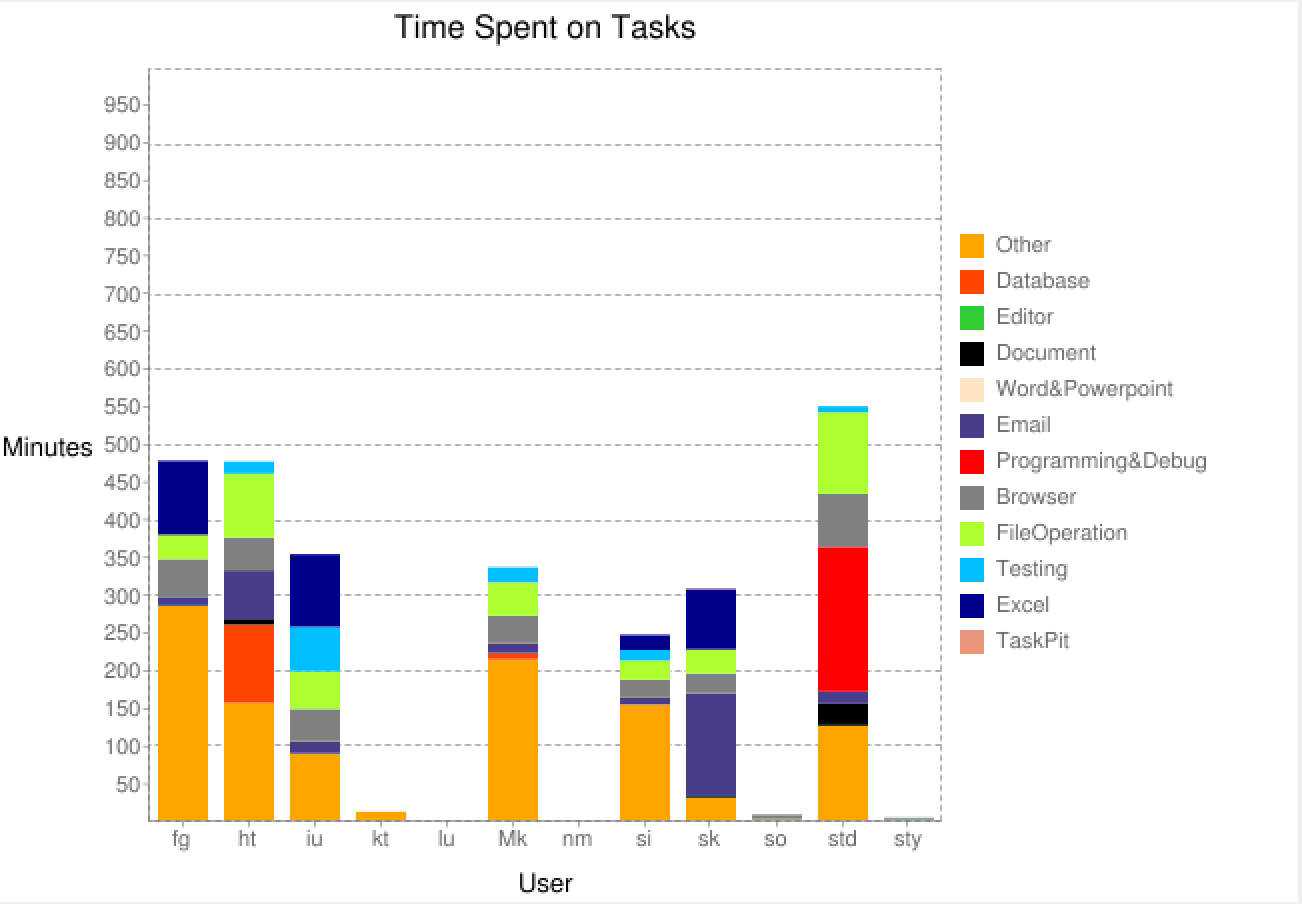
\includegraphics[width=0.5\textwidth]{fig1}
	\caption{Total time spent on tasks}
	\label{fig1}
\end{figure}

\begin{figure}[h]
	\centering	
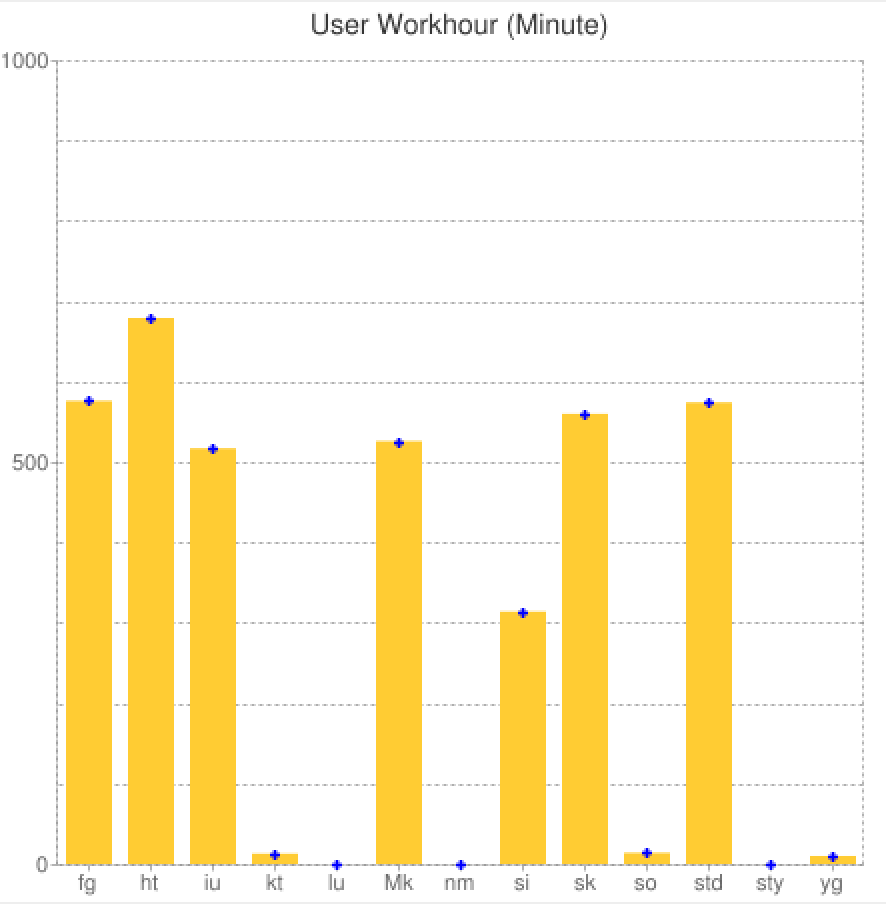
\includegraphics[width=0.3\textwidth]{fig2}
	\caption{Total work hour}
	\label{fig2}
\end{figure}

\begin{figure}[h]
	\centering	
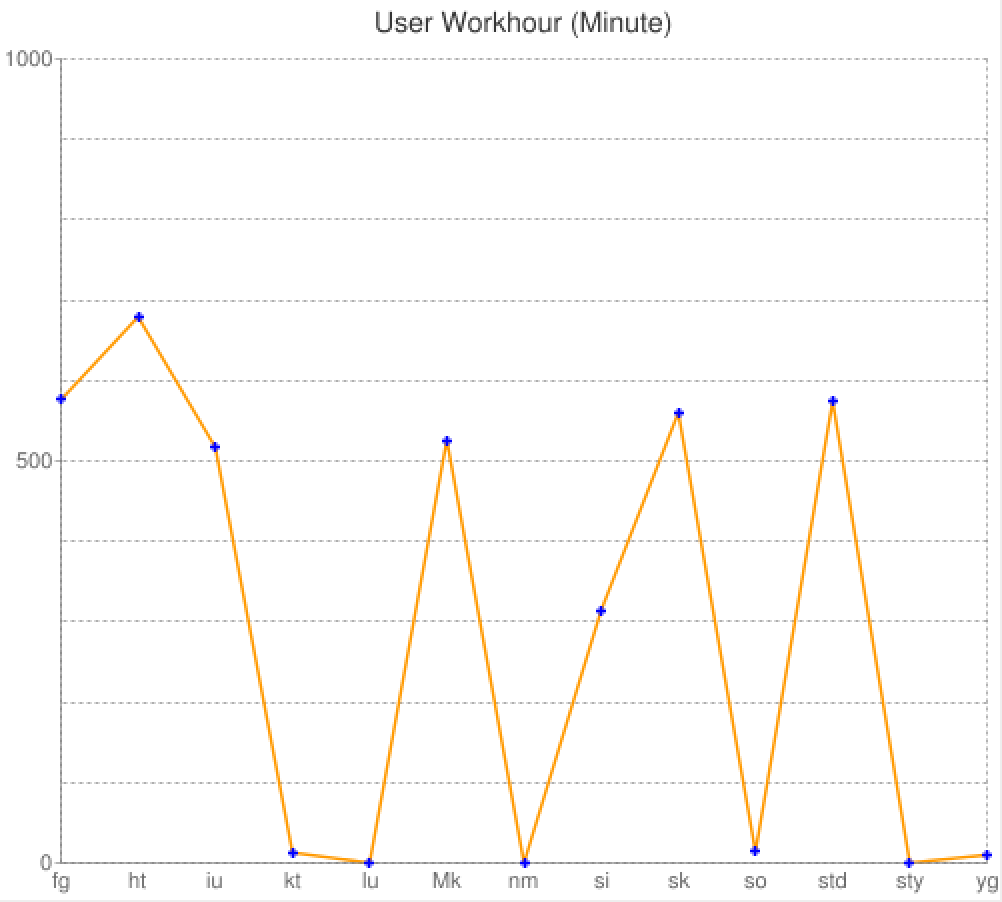
\includegraphics[width=0.3\textwidth]{fig3}
	\caption{Total work hour in Line Chart}
	\label{fig3}
\end{figure}
	
\subsection{System Design}
	As shown in Figure \ref{fig4}, TaskPit have its own database working at the back end of the system along with the visualization unit, configuration, and log files with daily report. In the configuration file will contain definitions of task and file as described before in the requirement section to be able to generate output of time interval of usage of each task and program in the log file. In Figure \ref{fig5} is the user interface of the program. Each task will record its own execution time by accumulating all time it has been in focus along with number of keystrokes and mouse clicks. \par
	To meet up the requirement of being less burden to the overall system and without providing server too much load, there will be a specified shared directory to store measurement result. Visualization tool is also used with configuration files and log files to graph visualize chart from various aspects of measurement results for specific period of time. Working in the client to server fashion as shown in Figure \ref{fig6}.
	
\begin{figure}[h]
	\centering	
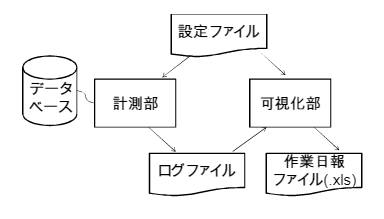
\includegraphics[width=0.3\textwidth]{fig4}
	\caption{Overall System}
	\label{fig4}
\end{figure}

\begin{figure}[h]
	\centering	
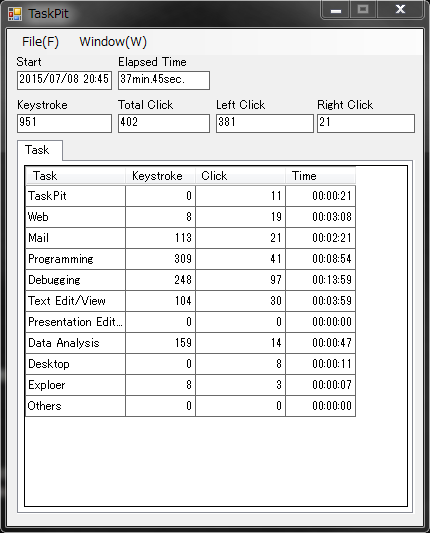
\includegraphics[width=0.3\textwidth]{fig5}
	\caption{TaskPit User Interface}
	\label{fig5}
\end{figure}

\begin{figure}[h]
	\centering	
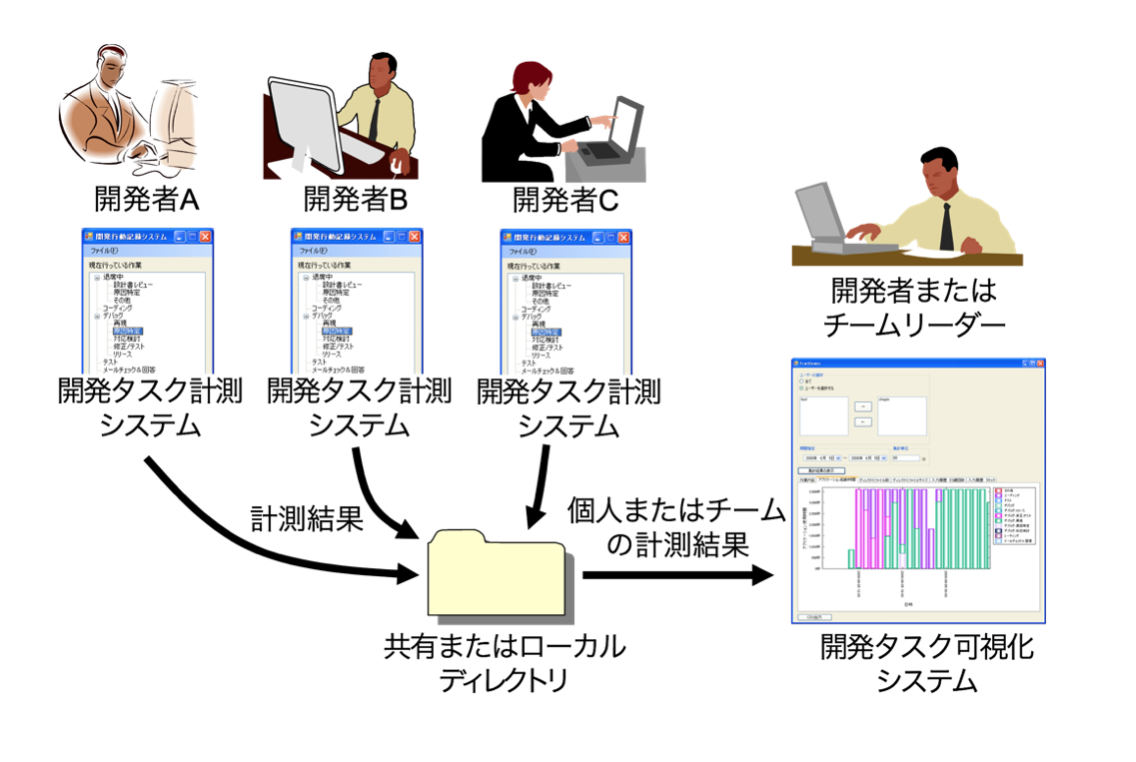
\includegraphics[width=0.3\textwidth]{fig6}
	\caption{Shared System}
	\label{fig6}
\end{figure}
	
\bibliography {taskpit}
\bibliographystyle {plain}
	
\end {document}